\chapter{Guide d'utilisation}
	\paragraph{} Apr\`es d\'eveloppement et d\'eploiement de notre solution, le site web \projectName\ fournira l'acc\`es aux illustrations de l'URG\'eo comme d\'ecrit ci-apr\`es. 
	
	\section{G\'erer les illustrations sur le site}
	 L'enregistrement des illustrations sur le site passe par l'ensemble des \'etapes interm\'ediares suivantes:
		 	\begin{itemize}
		 		\item[-] G\'erer des administrateurs
		 		\item[-] G\'erer des cat\'egories
		 		\item[-] G\'erer des \'etiquettes
		 		\item[-] G\'erer des auteurs
		 		\item[-] G\'erer des documents
		 		\item[-] G\'erer les listes de choix
		 	\end{itemize} 
	 	
	 	\paragraph{} Ces travaux ne peuvent \^etre r\'ealis\'es que par un utilisateur avec les droits d'administrateurs. Avant tout, l'utilisateur doit se connecter sur le dashboard comme suit.
	 	
		\subsection{Authentification}
			\fcolorbox{frameblue}{fillblue}{
				\begin{minipage}{6in}
					\begin{itemize}
						\item[-] Naviguer vers l'URL de la page de connection du dashboard(Voir Figure~\ref{FigLoginPage}) :\dashboardURL\
						\item[-] Entrer son nom d'utilisateur
						\item[-] Entrer son mot-de-passe
						\item[-] Cliquer sur le bouton 
\includegraphics[height=2ex]{Pictures/BoutonLogin.png} pour se connecter sur le dashboard(Voir Figure~\ref{FigDashboardRoot})
					\end{itemize}
				\end{minipage}
			}
		
				
		\begin{figure}
			\centering
			\begin{minipage}{0.45\textwidth}
				\centering
				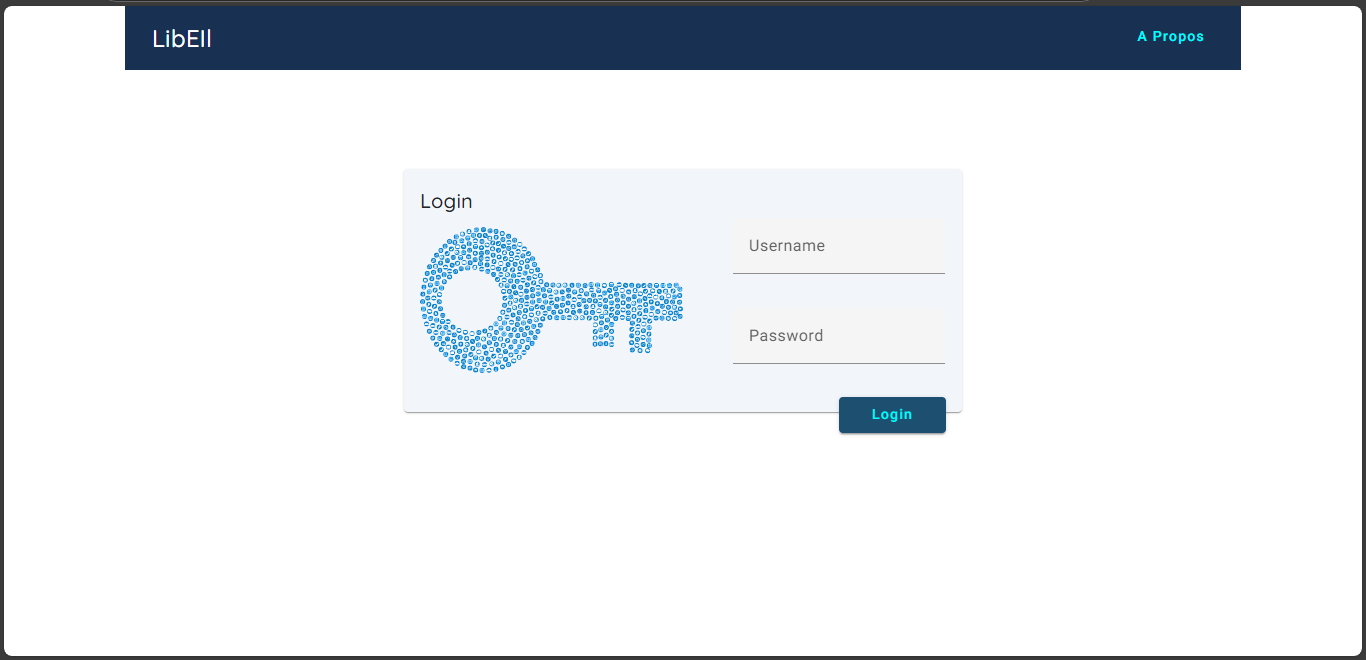
\includegraphics[width=\textwidth]{Pictures/PageDeConnection.png}
				\caption{Page de connection au dashboard}
				\label{FigLoginPage}
			\end{minipage}
			\hspace{5pt}
			\begin{minipage}{0.45\textwidth}
				\centering
				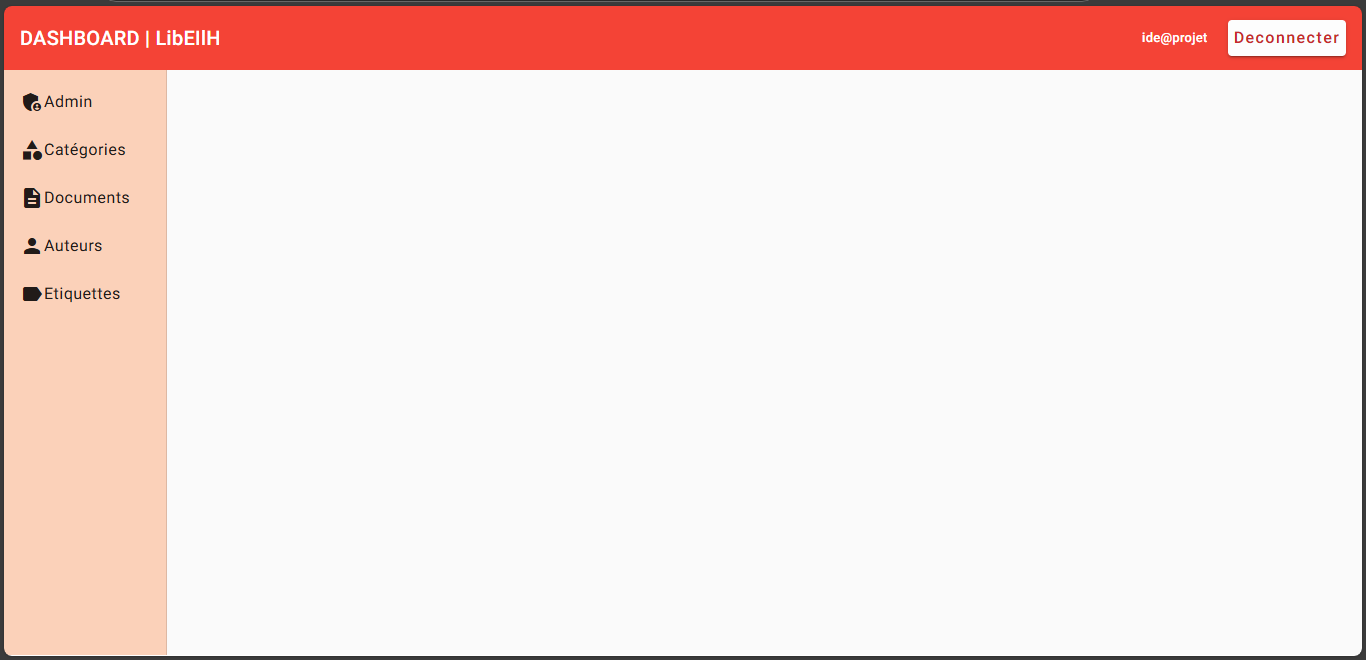
\includegraphics[width=\textwidth]{Pictures/Dashboard_rootPage.png}
				\caption{Page d'entr\'ee du dashboard}
				\label{FigDashboardRoot}
			\end{minipage}
		\end{figure}
		
		
		\paragraph{} Une fois connect\'e, l'administrateur choisit, dans la partie gauche de l'\'ecran, l'\'el\'ement \`a g\'erer.
		
		\begin{figure}[!ht]
			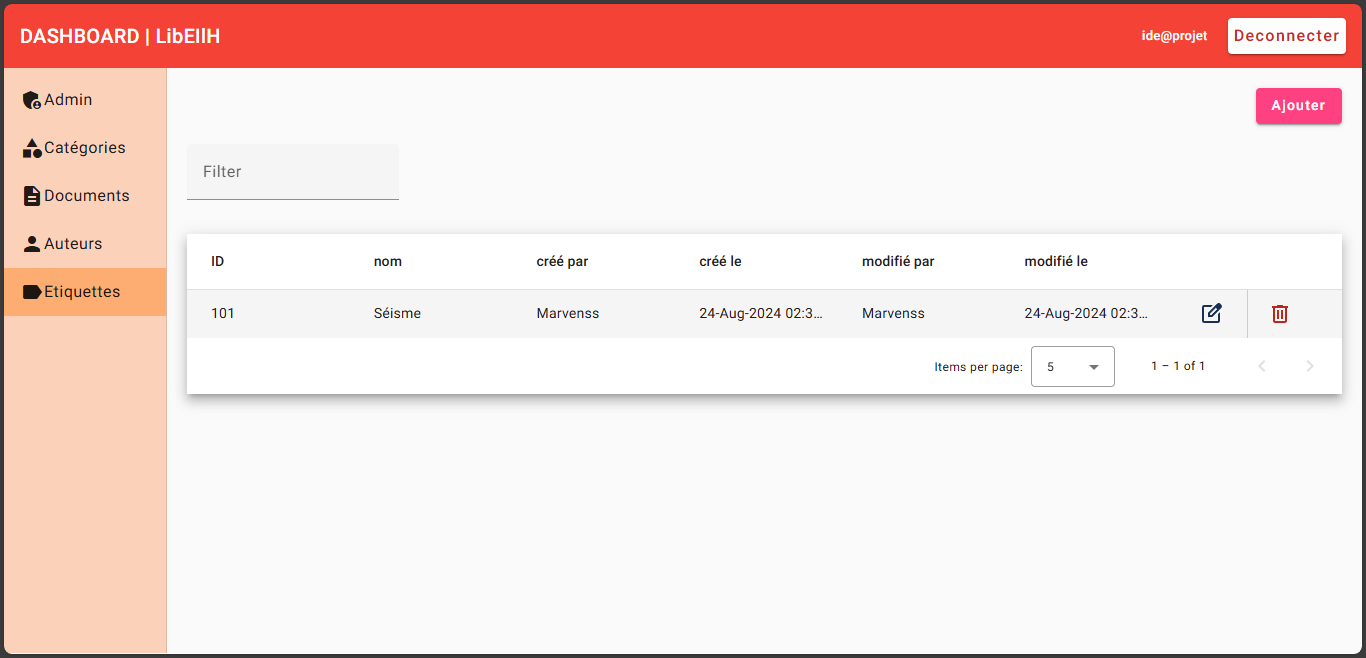
\includegraphics[width=0.5\textwidth]{Pictures/Dashboard_Etiquette.png}
			\centering
			\caption{Page de gestion des \'etiquettes}
			\label{FigChoixTypeElement}
		\end{figure}
		
		\paragraph{} Apr\`es avoir fait son choix (Voir Figure~\ref{FigChoixTypeElement}), l'utilisateur voit s'afficher la liste de tous les enregistrements de ce type dans la base de donn\'ees. Depuis cette page il est possible de supprimer ou modifier un enregistrement existant ou bien en ajouter un nouveau comme suit.
		
		\subsection{Ajouter}
			\fcolorbox{frameblue}{fillblue}{
				\begin{minipage}{6in}
					\begin{itemize}
						\item[-] Choisir le type d'\'el\'ement \`a ajouter 
						\item[-] Cliquer sur le bouton 
\includegraphics[height=2ex]{Pictures/BoutonAjouter.png} en haut \`a droite de l'\'ecran d'affichage
						\item[-] Remplir le formulaire d'ajout (Voir Figure~\ref{FigFormulaireAjouterDocument})
						\item[-] Cliquer sur le bouton 
\includegraphics[height=2ex]{Pictures/BoutonSoumettre.png}
					\end{itemize}
				\end{minipage}
			}
		
	 	
		
				
		\begin{figure}
			\centering
			\begin{minipage}{0.45\textwidth}
				\centering
				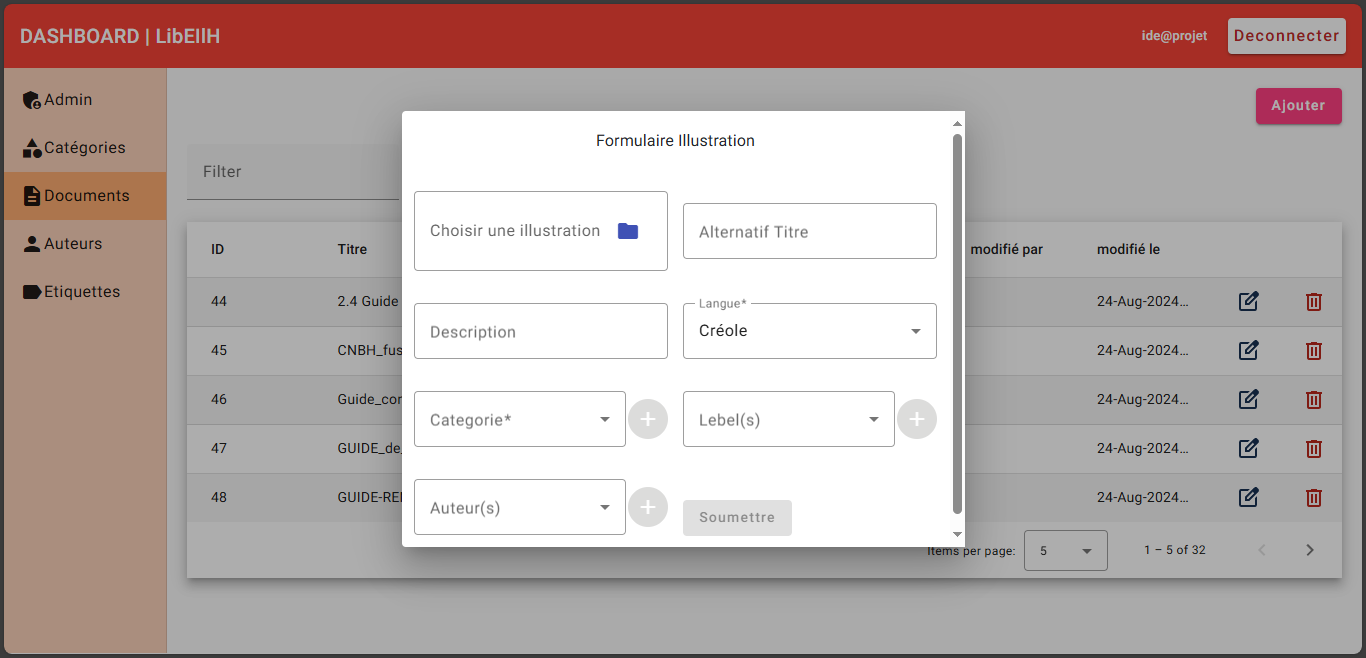
\includegraphics[width=\textwidth]{Pictures/Dashboard_AjouterDoc.png}
				\caption{Formulaire d'ajout de document}
				\label{FigFormulaireAjouterDocument}
			\end{minipage}
			\hspace{5pt}
			\begin{minipage}{0.45\textwidth}
				\centering
				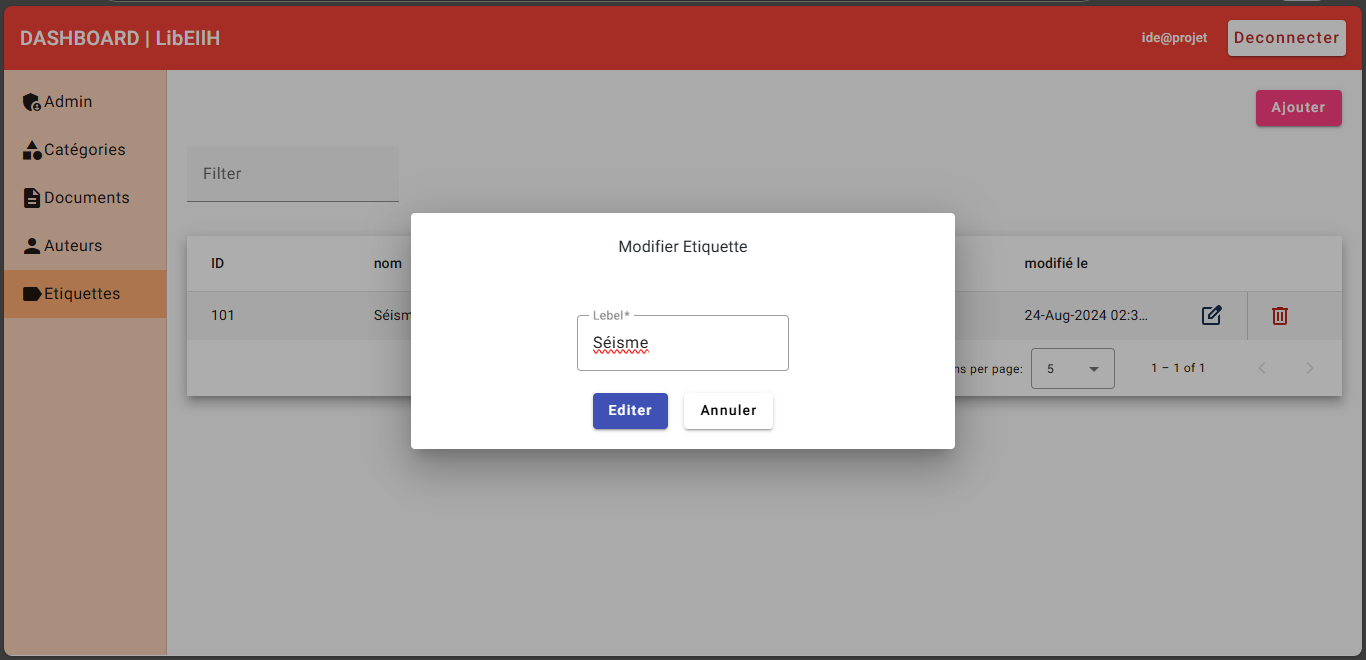
\includegraphics[width=\textwidth]{Pictures/Dashboard_ModifierEtiquette.png}
				\caption{Formulaire de modification d'un \'etiquette}
				\label{FigFormulaireModifierEtiquette}
			\end{minipage}
		\end{figure}
	 			


	 	\subsection{Modifier}
	 	\fcolorbox{frameblue}{fillblue}{
		 	\begin{minipage}{6in}
		 		\begin{itemize}
		 			\item[-] Choisir le type de l'\'el\'ement \`a modifier 
		 			\item[-] Cliquer sur l'ic\^one  
\includegraphics[height=2ex]{Pictures/BoutonModifier.png} correspondant \`a l'enregistrement \`a modifier
		 			\item[-] Remplir le formulaire de modification (Voir Figure~\ref{FigFormulaireModifierEtiquette})
		 			\item[-] Cliquer sur le bouton 
\includegraphics[height=2ex]{Pictures/BoutonSoumettre.png} 
		 		\end{itemize}
		 	\end{minipage}
	 }
 
		 \subsection{Supprimer}
		 \fcolorbox{frameblue}{fillblue}{
		 	\begin{minipage}{6in}
		 		\begin{itemize}
		 			\item[-] Choisir le type de l'\'el\'ement \`a supprimer 
		 			\item[-] Cliquer sur l'ic\^one  
\includegraphics[height=2ex]{Pictures/BoutonSupprimer.png} correspondant \`a l'enregistrement \`a supprimer
		 			\item[-] Confirmer l'action 
		 		\end{itemize}
		 	\end{minipage}
		 }
	 
 
	\section{Acc\'eder aux illustrations}
		Le site Web \projectName\ permet au simple\_utilisateur de:
		
		\begin{itemize}
			\item[-] Consulter une illustration
			\item[-] T\'el\'echarger une illustration
			\item[-] Visionner les informations relatives \`a une illustration
		\end{itemize} 
		
		
		\paragraph{} Pour acc\'eder aux ressources, l'utilisateur doit naviguer vers l'adresse web du site '\websiteURL\'. 
					
				
		\begin{figure}
			\centering
			\begin{minipage}{0.45\textwidth}
				\centering
				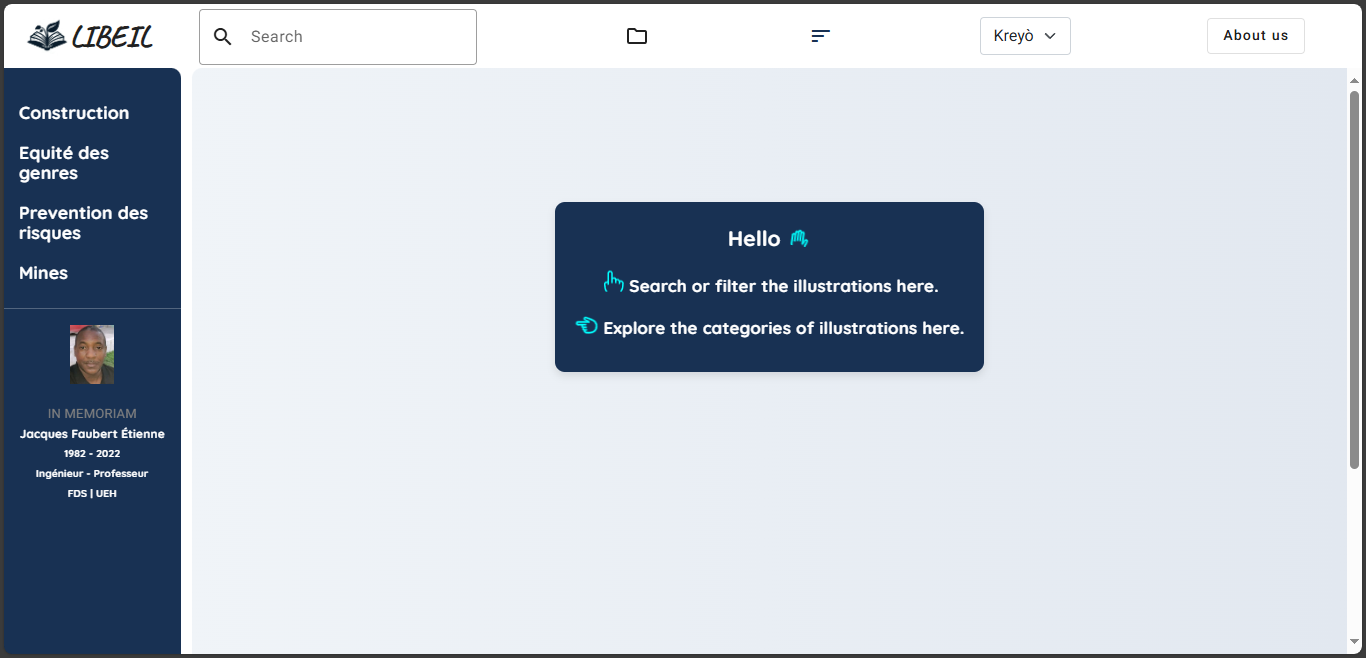
\includegraphics[width=\textwidth]{Pictures/PageDAccueil.png}
				\caption{Page d'accueil du site}
				\label{FigAccueilSU}
			\end{minipage}
			\hspace{5pt}
			\begin{minipage}{0.3\textwidth}
				\centering
				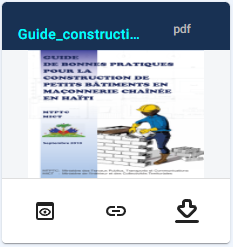
\includegraphics[height=4cm]{Pictures/IllustrationCard.png}
				\caption{Une illustration sur le site}
				\label{FigIllustrationCard}
			\end{minipage}
		\end{figure}
	
		\fcolorbox{frameblue}{fillblue}{
			\begin{minipage}{6in}
				Depuis la page d'accueil (Voir figure~\ref{FigAccueilSU}), il peut soit afficher les illustrations par cat\'egorie, soit rechercher des illustration suivant des mots cl\'es. Dans les deux cas il verra s'afficher un ensemble d'illustrations (Voir figure~\ref{FigIllustrationCard}) suivant la cat\'egorie de son choix ou les mots cl\'es de sa recherche.
				
				\paragraph{} De l\`a, pour chacune des illustrations affich\'ees, l'utilisateur peut choisir de:
				\begin{itemize}
					\item[-] faire un double-clique rapide dessus pour la consulter
					\item[-] cliquer sur l'ic\^one  
\includegraphics[height=2ex]{Pictures/BoutonDetails.png} pour en visionner les d\'etails
					\item[-] cliquer sur l'ic\^one 
\includegraphics[height=2ex]{Pictures/BoutonCopierLien.png} pour copier le lien vers cette illustration
					\item[-] cliquer sur l'ic\^one  
\includegraphics[height=2ex]{Pictures/BoutonDetails.png} pour la t\'el\'echarger
				\end{itemize}
			\end{minipage}
		}
 
	
 
			
		\begin{figure}[htb]
			\centering
			\begin{minipage}{0.45\textwidth}
				\centering
				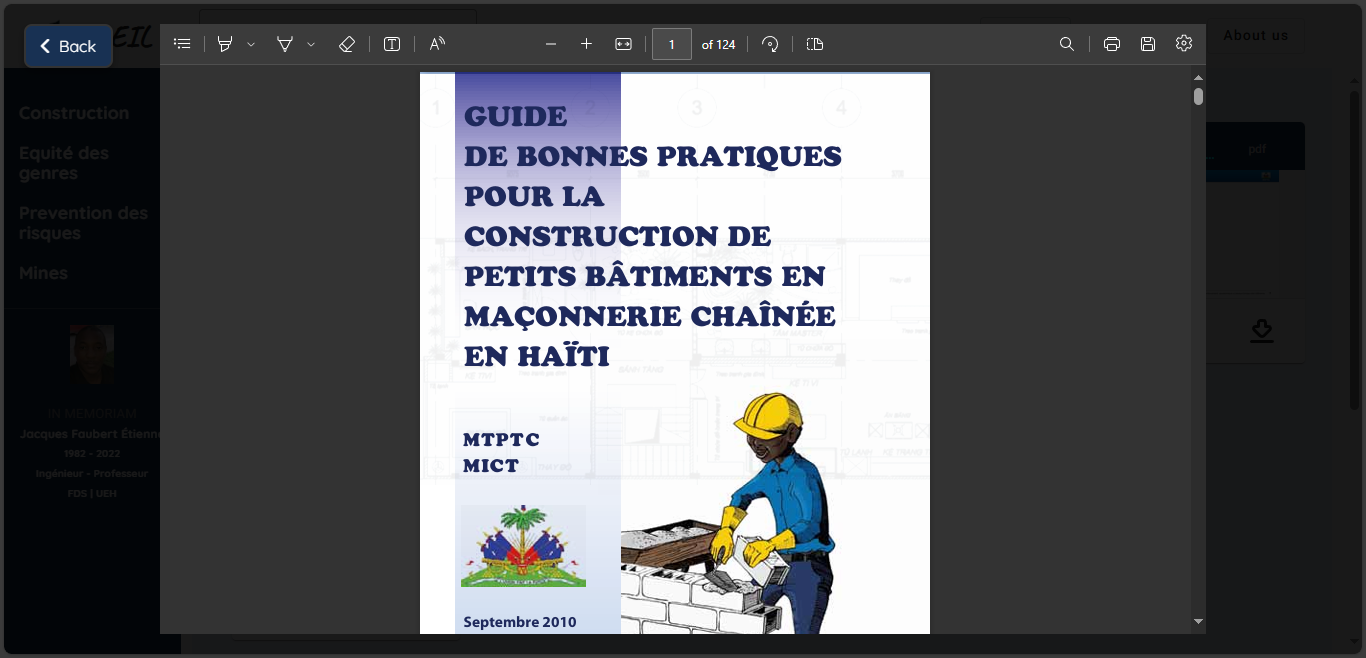
\includegraphics[width=\textwidth]{Pictures/PageDeConsultation.png} 
				\caption{Consultation d'une illustration pdf}
				\label{FigConsultationFleDize}
			\end{minipage}
			\hspace{5pt}
			\begin{minipage}{0.3\textwidth}
				\centering
				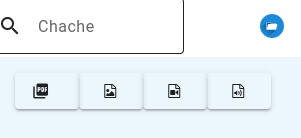
\includegraphics[width=0.8\textwidth]{Pictures/Filtre.png}
				\caption{Filtrage des illustrations suivant leur type de fichier}
				\label{FigFiltreIllustration}
			\end{minipage}
		\end{figure}
		
		\paragraph{} En plus des fonctionnalit\'es cit\'ees ci-dessus, le site fournit les suivantes:
		
		
		\fcolorbox{frameblue}{fillblue}{
			\begin{minipage}{6in}
			\begin{itemize}
				\item[-] Trie\\
						L'utilisateur peut trier les illustrations affich\'ees suivant le crit\`eres de son choix parmi la liste de crit\`eres disponible en appuyant sur 
\includegraphics[height=2ex]{Pictures/BoutonTrie.png} 
				\item[-] Filtre\\
						Le bouton 
\includegraphics[height=2ex]{Pictures/BoutonFiltre.png} (Voir figure~\ref{FigFiltreIllustration}) permet \`a l'utilisateur de filtrer les illustrations suivant leur type de fichier (document, audio, vid\'eo, image).
				\item[-] Langue d'affichage\\
						L'utilisateur peut choisir la langue de l'interface parmi le cr\'eole Ha\"itien, cite{}l'anglais, le fran\c{c}ais et l'espagnol en utilisant le bouton 
\includegraphics[height=2ex]{Pictures/BoutonLangue.png}
				\item[-] A propos\\
						L'utilisateur peut voir l'\'equipe de r\'ealisation du projet \projectName\ en cliquant sur 
\includegraphics[height=2ex]{Pictures/BoutonTelecharger.png}
			\end{itemize}
		\end{minipage}
	}

	
		\begin{figure}[htb]
			\centering
			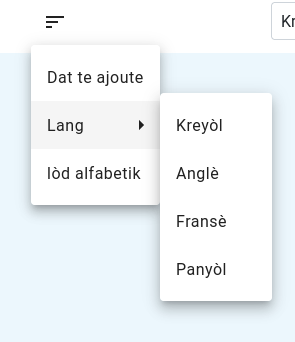
\includegraphics[width=0.8\textwidth]{Pictures/Trie.png}
			\caption{Filtrage des illustrations suivant leur type de fichier}
			\label{FigFiltreIllustration}
		\end{figure}
	



\chapter*{***}
	\addcontentsline{toc}{chapter}{***}
	
	Le projet \projectName\ visait \`a construire et mettre en production une solution permettant de rendre les illustrations de l'URG\'eo accessibles partout en Ha\"iti et \`a travers le monde dans le but d'\'eduquer la population sur plusieurs sujet mais surtout sur la gestion des risques. Apr\`es avoir fait l'\'etat des connaissances sur le domaine nous nous sommes propos\'e de construire un e-librairie distribu\'e via le site Web \projectName .
	\vspace{15pt}
	
	\paragraph{} Nous avons d\'evelopp\'e avec succ\`es une plate-forme Web performante et s\'ecuris\'ee qui permet de charger, de cat\'egoriser, de g\'erer et de distribuer les illustrations. \projectName centralise ainsi des informations fiables adapt\'ees \`a l'environnement Ha\"itien, faciles \`a comprendre, \`a interpr\'eter et \`a retenir sur des sujets cl\'es qui concernent des risques auxquelles la population Ha\"itienne locale fait face mais aussi le monde entier. Cela permettra de mieux comprendre ces risques, de mieux s'y pr\'eparer avant, de mieux y faire face, et de mieux r\'eparer les d\'egats qu'ils causent.\par
	\noindent Quand le projet aura grandit et devenu, nous l'\'esperons, une r\'ef\'erence pour trouver des informations sur les risques, on pourrait y impl\'ementer compl\`etement une conformit\'e de niveau deux ou de niveau 3 au Standard ASVS 4.0.3,  y int\'egrer la possibilit\'e pour les utilisateurs de donner leur avis sur la plateforme pour aider \`a l'am\'elioration de celui-ci et sur chaque document pour aider les auteurs \`a augmenter la qualit\'e et l'efficacit\'e de leur cr\'eation et \`a mieux adapter leur contenu. On pourrait y ajouter, aussi un forum qui permettrait d'aller plus en profondeur dans les connaissances \`a partager, ou d'\^etre plus sp\'ecifique dans la gestion des risques. Ou encore des nouvelles en temps r\'eel sur le d\'eveloppement des ph\'enom\`enes tels que la formation de temp\^etes, d'ouragan; les activit\'es sismiques enregistr\'es en Ha\"iti; etc. Les horizons sont infinis...
	\vspace{15pt}
	
	\paragraph{}La r\'ealisation de notre projet de fin d\'etude \`a \'et\'e pour nous comme une quatri\`eme ann\'ees de sp\'ecialisation, tant elle \'etait riche en apprentissage, que ce soit sur la gestion/r\'ealisation de projet, sur la documentation d'un projet en ex\'ecution, sur les risques en Ha\"iti ou sur certains parmi les diff\'erents outils et technologies que nous avons utilis\'es. Nous sommes contents et fiers d'avoir eu cette chance. Et nous le serons encore plus quant nous Notre pays sera un endroit o\`u il fait bon vivre et les crises et catastrophes \`a longueur de journ\'ee seront un mauvais souvenir et une bonne source de motivation. 